\section{Proposed Architecture}\label{sec:arch}

\subsection{Overview}
Figure~\ref{fig:arch} shows the design. Devices and a protocol gateway sit in the field zone; the zone PEP enforces decisions; the trust engine (policy decision point, PDP), trust oracle and a local replica of the chain state sit in the site operations zone; and the three contracts are operated by the consortium. The PEP/PDP split follows the classical Zero Trust reference model \cite{nist800207,fernandez2024critical}, but the policy store and the identity registry are held by the consortium rather than by one site, so that no gateway can edit another stakeholder's view of a device.

\begin{figure*}[t]
\centering
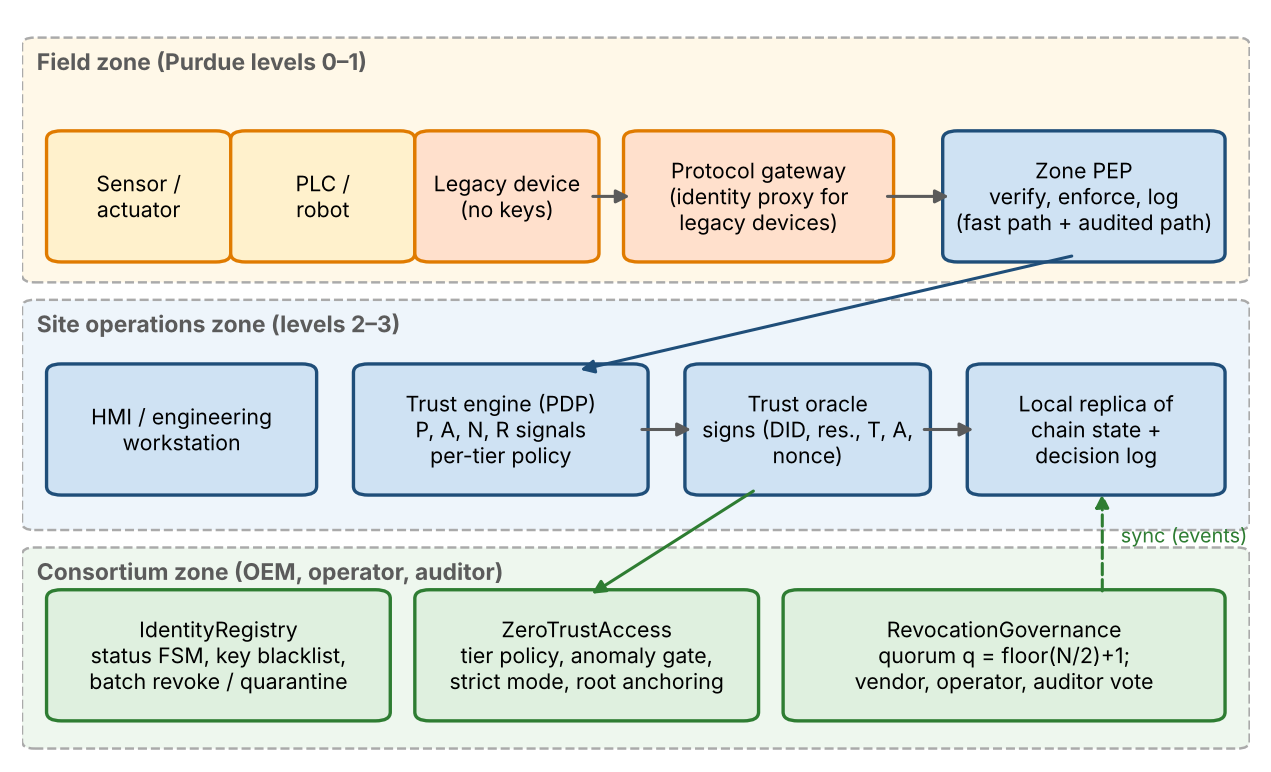
\includegraphics[width=0.62\textwidth]{../figures/fig7_iiot_arch.png}
\caption{Architecture of the blockchain-enabled Zero Trust system for Industrial IoT identity management, organized by plant zone.}
\label{fig:arch}
\end{figure*}

\subsection{Identity Lifecycle and the Registry}\label{sec:identity}
A device derives a DID from its public key in the style of the W3C data model \cite{w3cdid2022}, $\mathrm{did}=\texttt{did:iot:}\,\mathrm{H}(pk)[0{:}32]$, with SHA-256 in the testbed and Keccak-256 in the Solidity track. Commissioning submits $pk$ (or its hash), a device class, and a hash of the declared attributes (firmware version, vendor, location), signed by $sk$ so that the record proves key possession without exposing the attributes. The registry is a state machine:
\[
\text{UNKNOWN} \xrightarrow{\text{register}} \text{ACTIVE}
\]
\[
\text{ACTIVE} \xrightarrow{\text{suspend}} \text{SUSPENDED} \xrightarrow{\text{reinstate}} \text{ACTIVE}
\]
\[
\text{ACTIVE or SUSPENDED} \xrightarrow{\text{revoke}} \text{REVOKED (terminal)}
\]
REVOKED is terminal, and revocation also blacklists the key hash, so the same key cannot be enrolled under a new DID. Suspension is the reversible quarantine used while an advisory is assessed. All transitions are restricted to the registrar role and emit indexed events, which zone replicas and security monitoring consume.

\subsection{Legacy Devices Behind a Protocol Gateway}\label{sec:legacy}
Brownfield equipment often cannot sign requests. We represent each such device by a DID derived from the \emph{gateway's} key and the device's local address, registered with the class \texttt{legacy}. The gateway signs on its behalf and supplies weaker posture evidence (the testbed draws legacy posture from a lower range than native devices). Two rules keep this from lowering the security of the whole plant: the class check admits \texttt{legacy} identities only to low-consequence resources (tiers T0--T1 in our policy), and revoking the gateway key revokes every proxied identity at once. The trade-off is explicit: a compromised gateway can speak for every legacy device behind it, which is why this class never reaches the strict tiers.

\subsection{Tiered Zero Trust Policy}\label{sec:tiers}
Each resource has a policy $\pi=(\theta,m,g,s,\mathcal{C},\tau_{\max})$: a minimum trust $\theta$, a step-up margin $m$, an anomaly hard gate $g$, a strict flag $s$, a set of permitted device classes $\mathcal{C}$ and a maximum idle time $\tau_{\max}$. Table~\ref{tab:tiers} lists the four tiers used in our evaluation. The parameters are illustrative and tuned by hand to our synthetic signal ranges; a real plant would set them from its own telemetry and risk assessment.

\begin{table}[t]
\centering
\caption{Criticality tiers used in the evaluation}
\label{tab:tiers}
\scriptsize
\begin{tabular}{@{}llcccl@{}}
\toprule
\textbf{Tier} & \textbf{Example resource} & $\theta$ & $m$ & $g$ & \textbf{Classes} \\
\midrule
T0 & telemetry.read & 0.50 & 0.10 & 1.00 & all, incl.\ legacy \\
T1 & historian.write & 0.55 & 0.10 & 0.60 & all but HMI \\
T2 & plc.setpoint.write$^{\dagger}$ & 0.70 & 0.05 & 0.30 & HMI, PLC, robot \\
T3 & plc.firmware.update$^{\dagger}$ & 0.78 & 0.04 & 0.20 & PLC, robot \\
\bottomrule
\multicolumn{6}{l}{$^{\dagger}$ strict: borderline scores are denied rather than stepped up.}
\end{tabular}
\end{table}

The trust score combines four signals in $[0,1]$: device posture $P$ (attested firmware and configuration state), behavioural anomaly $A$, network context $N$ and historical reliability $R$ (mean of the last ten scores, 0.6 for a new device),
\begin{equation}
T=w_pP+w_b(1-A)+w_nN+w_rR,\label{eq:score}
\end{equation}
with default weights $(w_p,w_b,w_n,w_r)=(0.30,0.30,0.20,0.20)$,
\label{sec:signals}The signals come from the PEP and from monitoring that the plant already operates; in practice $A$ could be produced by process-aware anomaly detection, possibly trained across sites without sharing raw data \cite{tom2025flcti}. We treat their production as an input and evaluate only how the policy handles them. The oracle signs $(\mathrm{did},\mathrm{res},T,A,\mathrm{nonce})$; including $A$ in the signed message is what lets a contract enforce the gate without trusting the device's own report.

\begin{center}
\begin{minipage}{\linewidth}
\small
\textbf{Algorithm 1} \texttt{evaluateAccess(did, res, class, T, A, nonce, sig)}
\begin{enumerate}[leftmargin=1.4em,itemsep=0pt,topsep=2pt]
  \item \textbf{if} status(did) $\ne$ ACTIVE \textbf{or} no policy for res \textbf{then return} DENY
  \item \textbf{if} (did, nonce) already used \textbf{then return} DENY; mark it used
  \item \textbf{if} class $\notin\mathcal{C}$ \textbf{then return} DENY
  \item \textbf{if} oracle signature over (did, res, $T$, $A$, nonce) is invalid \textbf{then return} DENY
  \item \textbf{if} $A>g$ \textbf{then return} DENY \hfill\textit{(anomaly gate)}
  \item \textbf{if} $T<\theta$ \textbf{then return} DENY
  \item \textbf{if} $T<\theta+m$ \textbf{then return} (\textbf{if} strict \textbf{then} DENY \textbf{else} STEP\_UP)
  \item \textbf{return} ALLOW
\end{enumerate}
\end{minipage}
\end{center}

The gate and the strict flag address a specific weakness of weighted scores that Proposition~\ref{prop:bound} makes precise: because the score is linear, an attacker who spoofs posture, network and reliability can hold $T$ high no matter how abnormal its behaviour is, so for consequential resources the anomaly signal must be able to veto independently of the sum. For a step-up, we leave the second-factor mechanism to the plant (for example a local operator confirmation); STEP\_UP is never returned for strict resources.

\subsection{Hybrid Enforcement: Fast Path and Audited Path}\label{sec:hybrid}
Running Algorithm~1 on the chain for every request would cap throughput at what a block can carry and would couple plant operations to consensus latency. We therefore split enforcement by tier.
\begin{itemize}[leftmargin=1.1em,itemsep=0pt,topsep=1pt]
  \item \textbf{Fast path (T0, T1).} The zone PEP decides locally against its replica: status and key from the registry events, a per-device monotonic counter in place of the nonce set, the device's request signature, the oracle's attestation and the tier policy. Each decision appends a leaf to a log; every $B$ decisions the PEP computes a Merkle root and anchors it with \texttt{anchorDecisions(root, count)}, which only authorized PEP addresses may call. An auditor can later check any single logged decision against the anchored root.
  \item \textbf{Audited path (T2, T3).} The request is decided by \texttt{evaluateAccess} on the chain, so the decision, its inputs and its outcome are themselves on the ledger. These resources are written rarely and under operator control, which is what makes the cost acceptable; if a plant's setpoint writes are frequent, this assumption fails and the tiers must be re-cut.
\end{itemize}
The price of the fast path is the replica lag $\Delta$ of assumption A5: a device revoked just before a request may still be accepted for tier T0--T1 resources until the replica catches up (Proposition~\ref{prop:stale}). The audited path has no such window.

\subsection{Firmware Recall and Quarantine}\label{sec:recall}
When a vulnerability is disclosed in a firmware generation, the manufacturer needs to withdraw every affected device quickly. \texttt{revokeBatch(dids, reason)} revokes many devices in one transaction, skips unknown or already-revoked entries rather than reverting (so one stale entry cannot block a recall), blacklists each key and emits one event per device; \texttt{suspendBatch} quarantines them reversibly. The batch is limited by the block gas limit, and Section~\ref{sec:recall_eval} measures its per-device gas and the number of blocks needed for fleets of $10^3$--$5\times10^4$ devices.

\subsection{Decentralized Revocation Governance}\label{sec:governance}
A single registrar can deny service to legitimate devices, or reinstate a dangerous one. \texttt{RevocationGovernance} mediates \texttt{revokeDevice()} through threshold voting among $N$ independent voters, in the spirit of the voter group of \cite{kumar2026privacy}. A voter calls \texttt{propose(did, reason)}; each voter casts one \texttt{castVote(id, approve)}. The proposal executes the revocation as soon as approvals reach $q=\lfloor N/2\rfloor+1$, and is finalized as rejected once denials exceed $N-q$. The governance contract holds the registrar role on the registry; time-critical actions that a signed vendor bulletin pre-authorizes may use the direct path, so the two paths coexist. Votes are non-transferable, one per voter, and DENY votes never count toward approval.

\subsection{Degraded Operation During an Outage}\label{sec:outage}
If a PEP loses its replica feed, it must pick between availability and safety. Our policy is tier-dependent: T0--T1 requests continue against the last known state (accepting that a device revoked during the outage is not yet known), while audited-path requests (T2--T3) are \emph{denied}, because their decision needs the chain. This is fail-closed for consequential writes and fail-operational for reads; whether an operator accepts that trade is a plant decision, and Section~\ref{sec:outage_eval} quantifies it for a simple scenario.
